\subsection{Key Expansion (Key Schedule)}

\subsubsection*{Importance of Key Expansion in AES} 

The Advanced Encryption Standard (AES) heavily relies on the key expansion (or key schedule), 
a process that derives a series of round keys from the initial cipher key. 
This process ensures that each round uses a different key, 
greatly increasing the cipher's security. The key expansion process slightly differs 
based on the AES version (AES-128, AES-192, or AES-256), mainly in the number of rounds 
and the size of the key.

\subsubsection*{Main Algorithm of Key Expansion}
\label{sec:key-expansion}

First, the initial key is loaded into the first $N_k$ words of the key schedule, where $N_k$ depends 
on the key size $K_{len}$ and the number of rounds $N_r$: ($K_{len}$, $N_r$) = (128, 10), (192, 12), and (256, 14) 
for AES-128, AES-192, and AES-256, respectively \cite{Key_Collisions} (shown in Figure~\ref{fig:key_comb}). AES requires $N_r+1$ round keys, each round key is 
128 bits (16 bytes) in size, equivalent to four words $N_b$ from the key schedule. The key schedule in 
response generates a total of $N_b$×($N_r+1$) words\cite{NIST_AES}. \newline

For example, for AES-192, the key schedule generates 52 words in the key expansion, which equals 208 bytes (4 \textit{bytes per word} × 52 \textit{words}).
13 round keys are then extracted from these words - one for each of the 12 rounds plus the initial key addition ($N_r$ + 1 = 13).

\begin{figure}[h] % 'h' means place the figure here if possible
    \centering
    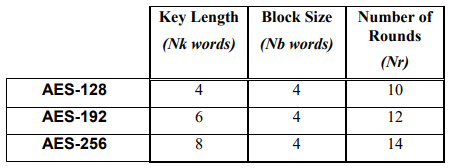
\includegraphics[width=.8\textwidth]{197_key_combinations.png} % Adjust width as needed
    \caption{
        Key-Block-Round Combinations \cite{NIST_AES}
    }
    \label{fig:key_comb} % Reference this figure with \ref{fig:sample_image}
\end{figure}

Then, the remaining words are generated iteratively. For words at positions that are a multiple of $N_k$, a 
transformation is applied to the previous word w[i-1] before the \Gls{XOR}. This transformation consists of RotWord 
followed by SubWord, and the result is then XORed with a round constant Rcon[i], where:

\begin{enumerate}
    \item \textbf{RotWord}: A cyclic permutation that shifts the bytes in the 4-byte input word one position to the left. 
    \item \textbf{SubWord}: A substitution operation that applies SubBytes operation to a 4-byte input word. 
    \item \textbf{Round Constant (Rcon)}:  An \Gls{XOR} operation with a round-dependent constant RC, where each Rcon[i]
    has a structure (RC[i], 0x00, 0x00, 0x00) \cite{NIST_AES}. 
\end{enumerate}

If the AES version is AES-256 ($N_k$ = 8) and i-4 is a multiple of $N_k$, the SubWord transformation is applied to the 
previous word (shown in Figure), but RotWord and Rcon are skipped. Otherwise, the new word is generated by XORing the previous word 
with the word $N_k$ positions earlier in the key schedule \cite{NIST_AES}. 

\begin{figure}[h] % 'h' means place the figure here if possible
    \centering
    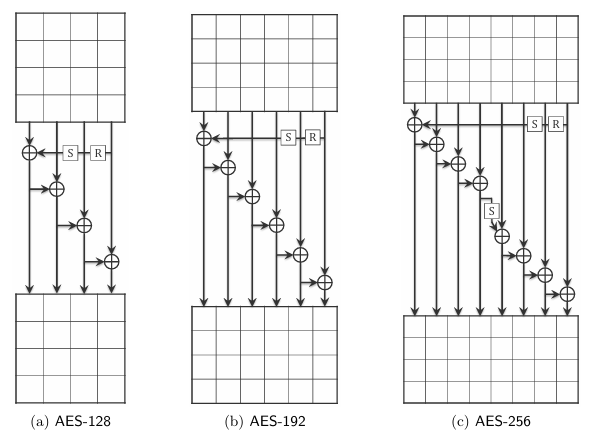
\includegraphics[width=.8\textwidth]{key_schedules.png} % Adjust width as needed
    \caption{
        Key schedules of AES-128, AES-192, and AES-256.The SubWord and
        RotWord functions are denoted by $S$ and $R$, respectively. Note that the round
        constant is not shown. \cite{Key_Collisions}
    }
    \label{fig:key_comb} % Reference this figure with \ref{fig:sample_image}
\end{figure}

\begin{figure}[h]
    \centering
    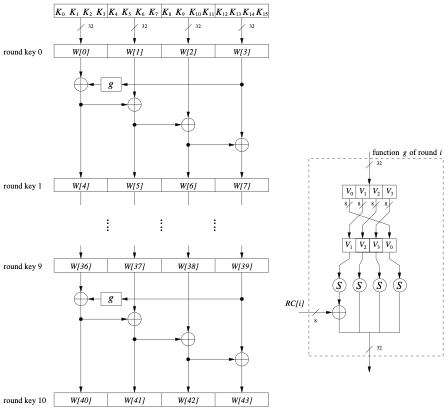
\includegraphics[width=.8\textwidth]{img/key-schedule-128.png}
    \caption{Key schedule for AES-128 \cite{Paar2024}.}
    \label{fig:key-schedule-128}
\end{figure}

\subsubsection*{Key Size and Security}

The key size directly impacts the security level of the algorithm, with 
longer keys providing higher security against brute force attacks. AES-128 offers sufficient security 
for most applications, but AES-192 and AES-256 are often preferred for applications requiring 
long-term security or protecting highly sensitive data. The increased number of rounds in AES-256 
further enhances its resistance against advanced cryptanalytic techniques.